%%%%%%%%%%%%%%%%%%%%%%%%%%%%%%%%%%%%%%%%%%%%%%%%%%%%%%%%%%%%%%%
% IMPORTANTE: Cambiar el compilador a XeLaTeX en las opciones %
%               Creditos Github: @diegocostares               %
%                Disponible en: @open-source-uc               %
%%%%%%%%%%%%%%%%%%%%%%%%%%%%%%%%%%%%%%%%%%%%%%%%%%%%%%%%%%%%%%%
\documentclass{style}

\begin{document}
%%%%%%%%%%%%%%%%% RENOMBRE %%%%%%%%%%%%%%%%%
\graphicspath{ {./img/} }
\renewcommand{\contentsname}{Índice de contenido}
\renewcommand{\listfigurename}{Índice de figuras}
\renewcommand{\listtablename}{Índice de Tablas}
\renewcommand{\tablename}{Tabla}
\renewcommand{\figurename}{Figura}
\renewcommand*{\lstlistingname}{Código}


%%%%%%%%%%%%%%%%% ENCABEZADO %%%%%%%%%%%%%%%%%
% Si se quiere eliminar, se tiene que quitar tambien las configuraciones del style.cls
\fancyhead[L]{ % Encabezado a la izquierda
  \begin{picture}(0,0) \put(-40,16){
\includegraphics[width=15mm]{img/logo-uc-3.pdf}} \end{picture}
  \put(8,40){\textcolor{gray}{\scriptsize{\begin{tabular}{l}
    PONTIFICIA UNIVERSIDAD CATÓLICA DE CHILE\\
    FACULTAD DE MATEMÁTICAS\\
    DEPARTAMENTO DE ESTADÍSTICA
  \end{tabular}}}}
}
\rhead{}


%%%%%%%%%%%%%%%%% PORTADA %%%%%%%%%%%%%%%%%
\begin{titlepage}

\includegraphics[width=2.5cm]{img/logo-uc-4.pdf} % AGREGAMOS EL LOGO UC
\vspace*{-2.8cm} % Esta linea va con la anterior


\begin{tabular}{l}
\hspace{2.5cm} PONTIFICIA UNIVERSIDAD CATÓLICA DE CHILE\\
\hspace{2.5cm} FACULTAD DE MATEMÁTICAS\\
\hspace{2.5cm} DEPARTAMENTO DE ESTADÍSTICA\\
\hspace{2.5cm} \underline{SEGUNDO SEMESTRE 2026}\\
\end{tabular}

\begin{center}
\vspace{3cm}
{\scshape\Huge \textbf{Predicción de la demanda eléctrica horaria a 24 horas} \par}
\rule{80mm}{0.1mm}

{\itshape\LARGE Alemania, España y Francia (2015--2019) \par}
\vfill
{\Large \textbf{EYP3407 - Tópicos Aplicados en Estadística} \par}
\medskip
{\large Trabajo final: análisis estadístico reproducible --- Caso 03 \par}
\bigskip
\begin{tabular}{cc}
    {\large \textbf{Profesor:}} & {\large \textbf{Ayudante:}} \\
    {\normalsize Eloy Alvarado} & {\normalsize Andrés Díaz} \\
\end{tabular}
\vspace{0.5cm}

{\Large \textbf{Grupo 03} \par}
\vspace{0.5cm}
{\large \textbf{Integrantes:}\\\normalsize Jorge Mardones, Diego Paredes, Matías Pineda, Benjamín Ruiz \par}

\medskip
\textbf{Fecha de entrega:} 10 de noviembre de 2026
\vspace{3cm}
\end{center}
\end{titlepage}
\newpage



%%%%%%%%%%%%%%%%% CONTENIDO %%%%%%%%%%%%%%%%%
\newpage
\section{Resumen}

\textbf{Problema.} Se estudia cuánto puede mejorarse una predicción estacional de la demanda eléctrica horaria a 24 horas en Alemania, España y Francia, con datos de 2015 a 2019 (ENTSO-E, vía Open Power System Data). La unidad es el par país--hora de emisión $t$ y la respuesta, la demanda en $t+24$.

\textbf{Diseño.} Se comparan dos referencias (persistencia y la misma hora de la semana anterior) con Ridge, un árbol podado y un Random Forest. La selección usa tres ventanas temporales expansivas dentro de 2015--2018 y 2019 se reserva para una única evaluación. La métrica es el NMAE macro (MAE de cada país relativo a su demanda media de entrenamiento, promediado).

\textbf{Resultado principal.} En 2019, el Random Forest con calendario cíclico obtiene un NMAE macro de 0,0249 frente a 0,0505 de la referencia semanal: 50,7\,\% menos error (IC 95\,\% por bloques semanales: 45,4\,\% a 54,9\,\%), con mejoras de 47\,\% a 54\,\% en cada país. También supera al árbol podado (25,1\,\%) y a Ridge (39,2\,\%). En el periodo de desarrollo (2015--2018) la mejora fue similar (49,6\,\%).

\textbf{Recomendación.} Usar el Random Forest, reajustado periódicamente con toda la historia, pues la ganancia se mantiene en la reserva y es clara frente a alternativas más simples.

\textbf{Limitaciones.} El modelo no incorpora feriados ni temperatura: en feriados el error diario llega a 11\,000 MW y la demanda se sobreestima, y en horas de alta demanda se subestima (sesgo de $-456$ a $-920$ MW). Los intervalos son condicionales al ajuste y a un solo año.

\section{Problema y datos}

\subsection{Pregunta, audiencia y decisión}

La pregunta es: \emph{¿cuánto puede mejorarse una predicción estacional de la demanda eléctrica horaria a 24 horas?} Es una \textbf{predicción sucesiva a horizonte fijo}: en cada hora de emisión $t$ se predice la demanda de $t+24$ con información disponible hasta $t$, y no equivale a emitir todo el día siguiente a una hora de mercado fija. La población son las tres series de demanda observada de Alemania (DE), España (ES) y Francia (FR) entre 2015 y 2019; la unidad es el par país--hora de emisión $t$ y la respuesta es la demanda en $t+24$, en MW.

El análisis se dirige a un operador del sistema eléctrico o a una comercializadora que programa con un día de anticipación la energía de cada hora; la decisión es cuánta energía programar o comprar para cada hora del día siguiente, y la referencia estacional semanal (repetir la demanda de la misma hora de la semana anterior) es la alternativa simple de comparación. Como equivocarse cuesta en ambos sentidos, se informan también el sesgo y el error por subgrupos. Las conclusiones son predictivas, sin interpretación causal.

\subsection{Procedencia y calidad de los datos}

Se usa el paquete entregado (\texttt{caso03\_demanda\_electrica.zip}), basado en \textit{Open Power System Data} (OPSD), serie horaria, versión 2020-10-06, cuyo origen es la plataforma de transparencia de ENTSO-E (Open Power System Data, 2020; ENTSO-E, s.\,f.). El archivo original (sin modificar) tiene 43\,824 horas y cinco columnas: dos marcas temporales (UTC y CET/CEST) y la demanda observada (MW) de DE, ES y FR. OPSD no declara una licencia explícita en sus metadatos; los datos se usan solo con fines académicos, citando al productor. \pend{PENDIENTE: Confirmar las condiciones de reutilización de ENTSO-E Transparency en su sitio y citarlas.} La auditoría mostró:
\begin{itemize}
    \item \textbf{Regularidad:} sin marcas temporales duplicadas ni saltos distintos de una hora, sin valores no positivos y con rangos plausibles (DE: 31\,307--77\,549 MW; ES: 17\,168--41\,015 MW; FR: 30\,426--94\,492 MW).
    \item \textbf{Ausentes:} DE, 0; ES, 18 (0,041\,\%); FR, 30 (0,068\,\%). No son ceros y se conservan como ausentes; su causa se desconoce, por lo que no se asumen aleatorios.
    \item \textbf{Zona horaria:} el orden y las particiones usan UTC y el calendario se deriva de la hora local del objetivo (\texttt{Europe/Berlin}, \texttt{Europe/Madrid}, \texttt{Europe/Paris}); como la clave es UTC, no hay horas repetidas ni ausentes por el cambio de horario.
\end{itemize}

\subsection{Construcción de la muestra} \label{sec:muestra}

La base se transforma a formato largo, con una fila por país--hora de emisión $t$ (llave: país y marca UTC, sin duplicados), y la respuesta es la demanda en $t+24$ obtenida por unión según país e instante objetivo. El periodo se asigna según el año de $t$. Las 24 horas del 31 de diciembre de 2018 quedan fuera, porque su respuesta cae en 2019, que se reserva. La figura \ref{img:flujo} resume el flujo y la tabla \ref{tab:muestra} entrega los tamaños.

\begin{figure}[!htbp]
    \centering
        \caption{Flujo de construcción de la muestra (filas país--hora).\label{img:flujo}}
        \begin{tikzpicture}[
            caja/.style={draw, rounded corners=2pt, align=center, font=\footnotesize, inner sep=3pt, text width=3.6cm},
            ancha/.style={draw, rounded corners=2pt, align=center, font=\footnotesize, inner sep=3pt, text width=11.6cm},
            flecha/.style={-{Stealth[length=2mm]}, thick}]
            \node[ancha] (raw) {\textbf{Archivo original:} 43\,824 horas $\times$ 5 columnas; 48 valores ausentes de demanda (ES: 18, FR: 30)};
            \node[ancha, below=3mm of raw] (largo) {\textbf{Formato largo país--hora:} $3 \times 43\,824 = 131\,472$ filas. Respuesta $Y_{t+24}$ y predictores calculados en UTC};
            \node[caja, below=4mm of largo] (dev) {\textbf{Periodo de desarrollo}\\$t$ en 2015--2018\\105\,120 filas};
            \node[caja, left=3mm of dev] (exc) {\textbf{Excluidas}\\$t$ el 31-dic-2018\\(respuesta en 2019)\\72 filas};
            \node[caja, right=3mm of dev] (res) {\textbf{Reserva}\\$t$ en 2019\\26\,280 filas};
            \node[caja, below=4mm of dev] (devc) {Casos completos\\(10 predictores y respuesta)\\103\,680};
            \node[caja, below=4mm of res] (resc) {Casos completos\\26\,031};
            \draw[flecha] (raw) -- (largo);
            \draw[flecha] (largo.south) -- ++(0,-2mm) -| (exc.north);
            \draw[flecha] (largo.south) -- (dev.north);
            \draw[flecha] (largo.south) -- ++(0,-2mm) -| (res.north);
            \draw[flecha] (dev) -- (devc);
            \draw[flecha] (res) -- (resc);
        \end{tikzpicture}
\end{figure}

\begin{table}[!htbp]
    \centering
        \caption{Construcción de la muestra por periodo y país (filas país--hora).\label{tab:muestra}}
        \footnotesize
        \begin{tabular}{llrrr}
\toprule
Periodo (según año del origen) & País & Orígenes & Con respuesta & Casos completos \\
\midrule
Periodo de desarrollo (2015--2018) & DE & 35\,040 & 35\,040 & 34\,873 \\
 & ES & 35\,040 & 35\,023 & 34\,651 \\
 & FR & 35\,040 & 35\,016 & 34\,156 \\
\midrule
Reserva (2019) & DE & 8\,760 & 8\,736 & 8\,736 \\
 & ES & 8\,760 & 8\,736 & 8\,736 \\
 & FR & 8\,760 & 8\,731 & 8\,559 \\
\midrule
Excluidos (31-dic-2018) & DE & 24 & 24 & -- \\
 & ES & 24 & 24 & -- \\
 & FR & 24 & 24 & -- \\
\bottomrule
\end{tabular}
    \\ Casos completos: respuesta y los diez predictores disponibles.
\end{table}

No se imputa: el entrenamiento y la evaluación de cada ventana usan solo \textit{casos completos}, para comparar todos los procedimientos sobre una base común. En el periodo de desarrollo (2015--2018) se pierden 167 filas en DE (0,48\,\%), 389 en ES (1,11\,\%) y 884 en FR (2,52\,\%), incluidas las primeras 167 horas de cada país (sin 168 horas de historia para la media móvil semanal). Una hora ausente deja sin respuesta a la fila $h-24$ y sin predictores completos a las filas desde $h$ en adelante, de modo que pocas horas ausentes eliminan muchas filas; las de ES caen todas en 2015 y las de FR en seis bloques, el mayor de 13 horas (anexo, tabla \ref{tab:ausentes_bloques}). Evaluar solo las fechas en que los tres países tienen caso completo cambia el NMAE por país a lo más 1,9\,\% y el macro a lo más 0,6\,\% (anexo, tabla \ref{tab:ausentes_efecto}), aunque no se puede descartar que las ausentes sean sistemáticas.

\subsection{Respuesta y predictores admisibles}

La respuesta se describe en el anexo (tabla \ref{tab:respuesta} y figura \ref{img:descriptiva}): las escalas difieren (España es casi la mitad de Alemania o Francia), por lo que las métricas agregadas se normalizan con la demanda media de entrenamiento de cada país; y hay un ciclo diario marcado, una caída los fines de semana y estacionalidad anual (más marcada en Francia), estructura que aprovechan las referencias estacionales y los rezagos de 24 y 168 horas.

Un predictor es admisible si se conoce en $t$: la demanda histórica hasta $t$ y el calendario local del instante $t+24$, que es determinista. Los rezagos se nombran por su distancia al \textit{instante objetivo}: \texttt{lag\_48h} es la demanda en $t-24$, \texttt{lag\_72h} la de $t-48$ y \texttt{lag\_168h} la de $t-144$ (la misma hora de la semana anterior al objetivo). Las medias móviles usan solo horas hasta $t$. La tabla \ref{tab:variables} resume la decisión sobre cada variable. \texttt{target\_is\_weekend} no es predictor porque se deriva de \texttt{target\_day}; se usa solo en el diagnóstico. No hay feriados ni variables meteorológicas, pues el caso exige trabajar solo con los archivos entregados.

\begin{table}[!htbp]
    \centering
        \caption{Variables admisibles y excluidas.}
        \footnotesize
        \label{tab:variables}
        \renewcommand{\arraystretch}{1.1}
        \begin{tabular}{@{}p{4.6cm}p{5.4cm}p{1.9cm}p{1.9cm}p{1.9cm}@{}}
            \toprule
            Variable & Interpretación & Tipo & Disponibilidad & Decisión \\
            \midrule
            \texttt{country} & País (DE, ES, FR) & categórica & siempre & incluida \\
            \texttt{demand\_mw} & Demanda en la hora de emisión $t$ & numérica, MW & en $t$ & incluida \\
            \texttt{lag\_48h}, \texttt{lag\_72h}, \texttt{lag\_168h} & Demanda en $t-24$, $t-48$ y $t-144$ & numérica, MW & en $t$ & incluidas \\
            \texttt{rolling\_mean\_24h}, \texttt{rolling\_mean\_168h} & Media de la demanda de las 24 y 168 horas hasta $t$ & numérica, MW & en $t$ & incluidas \\
            \texttt{target\_hour}, \texttt{target\_day}, \texttt{target\_month} & Hora (0--23), día de la semana y mes locales del objetivo & categóricas & calendario & incluidas \\
            \midrule
            \texttt{target\_demand\_mw} & Demanda en $t+24$ & numérica, MW & posterior a $t$ & respuesta \\
            \texttt{utc\_timestamp}, \texttt{target\_timestamp}, \texttt{cet\_cest\_timestamp} & Claves temporales (emisión, objetivo) y hora CET/CEST original (no es la hora local) & fecha-hora & -- & identificadores; CET/CEST descartada \\
            \texttt{target\_is\_weekend} & Fin de semana del objetivo & lógica & calendario & excluida (derivada) \\
            \texttt{period}, \texttt{has\_*}, \texttt{last\_available\_timestamp}, \texttt{target\_outside\_dataset}, \texttt{time\_diff} & Marcadores de periodo, disponibilidad y auditoría (usan el fin de la base) & auxiliares & -- & excluidas \\
            \bottomrule
        \end{tabular}
\end{table}

\section{Diseño de evaluación}

\subsection{Particiones, información disponible y referencia}

Los datos se dividen en \textbf{periodo de desarrollo} (horas de emisión $t$ de 2015 a 2018), donde se entrena, valida y selecciona, y una \textbf{reserva} (2019) que no interviene en ninguna decisión. Dentro del periodo de desarrollo (2015--2018) se usan tres ventanas de origen creciente (figura \ref{img:ventanas}, tabla \ref{tab:ventanas}), que respetan el orden temporal (Bergmeir \& Benítez, 2012; Hyndman \& Athanasopoulos, 2021).

\begin{figure}[!htbp]
    \centering
        \caption{Esquema temporal de las particiones. Azul: entrenamiento. Naranja: validación. Gris: reserva usada una sola vez. La franja de 24 horas antes de cada validación no entra al entrenamiento.}
        \label{img:ventanas}
        \begin{tikzpicture}[x=2.4cm, y=0.5cm, font=\footnotesize,
            ent/.style={fill=RoyalBlue!70, draw=white, minimum height=4.5mm, inner sep=0pt},
            val/.style={fill=amarillo2, draw=white, minimum height=4.5mm, inner sep=0pt},
            res/.style={fill=silver, draw=white, minimum height=4.5mm, inner sep=0pt}]
            \foreach \a in {0,...,5} \draw[gray] (\a,0.2) -- (\a,-0.2);
            \foreach \a/\t in {0.5/2015,1.5/2016,2.5/2017,3.5/2018,4.5/2019} \node at (\a,0.6) {\t};
            \draw[gray] (0,0) -- (5,0);
            \node[anchor=east] at (-0.1,-1) {W1};
            \node[ent, anchor=west, minimum width=0.99*2.4cm] at (0,-1) {entrenamiento};
            \node[val, anchor=west, minimum width=0.99*2.4cm] at (1,-1) {validación};
            \node[anchor=east] at (-0.1,-2) {W2};
            \node[ent, anchor=west, minimum width=1.99*2.4cm] at (0,-2) {entrenamiento};
            \node[val, anchor=west, minimum width=0.99*2.4cm] at (2,-2) {validación};
            \node[anchor=east] at (-0.1,-3) {W3};
            \node[ent, anchor=west, minimum width=2.99*2.4cm] at (0,-3) {entrenamiento};
            \node[val, anchor=west, minimum width=0.99*2.4cm] at (3,-3) {validación};
            \node[anchor=east, align=right] at (-0.1,-4) {Final};
            \node[ent, anchor=west, minimum width=3.99*2.4cm] at (0,-4) {reajuste con 2015--2018};
            \node[res, anchor=west, minimum width=0.99*2.4cm] at (4,-4) {prueba 2019};
        \end{tikzpicture}
\end{figure}

\begin{table}[!htbp]
    \centering
        \caption{Ventanas de validación temporal y tamaños (casos completos, suma de los tres países).}
        \label{tab:ventanas}
        \small
        \begin{tabular}{lllrr}
\toprule
Ventana & Entrenamiento (año de $t$) & Validación (año de $t$) & $n$ entrenamiento & $n$ validación \\
\midrule
W1 & 2015 & 2016 & 25\,484 & 26\,352 \\
W2 & 2015--2016 & 2017 & 51\,836 & 26\,087 \\
W3 & 2015--2017 & 2018 & 77\,923 & 25\,685 \\
\bottomrule
\end{tabular}
\end{table}

\textbf{Control de fuga.} Una fila de entrenamiento exige que su instante objetivo sea anterior a la primera hora de validación, de modo que su respuesta ya fuera conocida al emitir la primera predicción de validación; así se excluyen 24 filas por ventana. Estandarización, codificación y poda se ajustan solo con el entrenamiento de cada ventana. Los hiperparámetros se eligen con las tres ventanas de validación, por lo que el error allí es optimista; la estimación para datos nuevos es la de la reserva.

\textbf{Evaluación final.} Fijado todo, se reajusta con los 103\,680 casos completos de 2015--2018 y se evalúa una sola vez en 2019. Se informan los seis procedimientos, sin usarlos para elegir nada; el Random Forest cíclico es la versión final por la sensibilidad S1 (sección \ref{sec:sens}).

\textbf{Referencias.} \emph{Persistencia}, $\widehat Y_{t+24}=Y_t$, y \emph{estacionalidad semanal}, $\widehat Y_{t+24}=Y_{t+24-168}$ (misma hora de la semana anterior al objetivo); ninguna estima parámetros. En el periodo de desarrollo (2015--2018) la semanal (NMAE macro 0,0537) supera a la persistencia (0,0679) y queda fijada como referencia, aunque en Francia ocurre lo contrario (0,0573 frente a 0,0698).

\subsection{Métricas}

La métrica principal es el \textbf{NMAE macro}: para el país $c$ y la ventana $w$,
\begin{equation}
    \mathrm{NMAE}_{c,w}=\frac{\mathrm{MAE}_{c,w}}{\overline{Y}_{c,\mathrm{train}(w)}},\qquad
    \mathrm{NMAE}^{\mathrm{macro}}_{w}=\frac{1}{3}\sum_{c\in\{\mathrm{DE},\mathrm{ES},\mathrm{FR}\}}\mathrm{NMAE}_{c,w},
\end{equation}
con $\overline{Y}_{c,\mathrm{train}(w)}$ la demanda media de la respuesta en el entrenamiento de la ventana (en la reserva, del entrenamiento final). La normalización permite promediar países de escala distinta, y se elige el MAE por su lectura directa en MW y su menor sensibilidad a extremos. Como métricas complementarias se informan MAE y RMSE por país. No se usa MAPE porque pondera más los errores en horas de baja demanda. Todos los procedimientos se evalúan sobre las mismas filas completas de cada ventana; los denominadores están en las tablas de resultados y en el anexo (tabla \ref{tab:ausentes_efecto}).

\subsection{Errores detectados y correcciones}

Para evitar fuga se excluyeron las 24 horas de emisión del 31-dic-2018, se exigió objetivo anterior al inicio de cada validación y los normalizadores se calcularon solo con entrenamiento. Se detectaron y corrigieron errores de interpretación y de redacción que no modifican ninguna cifra: en borradores del informe (un ejemplo de propagación de ausentes invertido, un doble conteo de 167 horas, un pie de figura contrario a los datos y una justificación errónea sobre MAPE) y en dos notas de la síntesis del análisis de 2019 (una indicaba que las horas del 31-dic-2018 se usaron en validación, lo que contradice los 8\,736 orígenes por país de W3; otra decía que se sobreestiman los días posteriores a un feriado, cuando se subestiman).

\section{Métodos}

\subsection{Expectativas, preprocesamiento y presupuesto de búsqueda}

Antes del ajuste se formuló una expectativa por procedimiento. \textbf{Persistencia} y \textbf{estacional semanal} capturan los ciclos diario y semanal, pero fallan en transiciones entre laborables y fin de semana y con feriados. \textbf{M1, Ridge}: relación lineal y aditiva entre rezagos, medias móviles y calendario, sin interacciones (hora $\times$ tipo de día). \textbf{M2, árbol podado}: captura interacciones y no linealidades, pero es inestable y constante por tramos. \textbf{M3, Random Forest}: reduce la varianza del árbol, con mejor desempeño esperado, mayor costo y menor interpretabilidad; al ser por tramos, no extrapola niveles fuera del rango de entrenamiento.

\textbf{Preprocesamiento.} \texttt{country} y el calendario (\texttt{target\_hour}, \texttt{target\_day}, \texttt{target\_month}) se codifican con indicadores; las categorías no vistas en el entrenamiento se codifican con ceros. Ridge estandariza los seis predictores numéricos; árbol y bosque usan variables sin escalar. Todo es un \textit{pipeline} reajustado en cada ventana solo con el entrenamiento, con un modelo por procedimiento para los tres países. En la variante cíclica del Random Forest (M3$^\ast$, sección \ref{sec:sens}) hora, día y mes se reemplazan por pares seno--coseno con periodos 24, 7 y 12, y solo \texttt{country} usa indicadores; el resto y los hiperparámetros son los de M3.

\textbf{Presupuesto de búsqueda.} La tabla \ref{tab:busqueda} resume los modelos. Cada familia usa a lo más 20 configuraciones, evaluadas en las tres ventanas y elegidas por menor NMAE macro promedio.

\begin{table}[!htbp]
    \centering
        \caption{Procedimientos de aprendizaje, hiperparámetros y presupuesto de búsqueda.}
        \label{tab:busqueda}
        \small
        \renewcommand{\arraystretch}{1.1}
        \begin{tabular}{@{}p{2.6cm}p{3.3cm}p{5.6cm}p{1.2cm}p{2.5cm}@{}}
            \toprule
            Procedimiento & Modelo & Hiperparámetros evaluados & N.º config. & Selección \\
            \midrule
            M1: Ridge & Regresión lineal con penalización $\ell_2$ & $\alpha\in$ 15 valores logarítmicos entre $10^{-3}$ y $10^{4}$ & 15 & $\alpha=316{,}2$ \\
            M2: Árbol podado & Árbol de regresión con poda por costo--complejidad & \texttt{ccp\_alpha}: 20 valores de la ruta de poda del árbol completo & 20 & \texttt{ccp\_alpha}$=256{,}9$ \\
            M3: Random Forest & Bosque de 200 árboles & \texttt{max\_depth}$\in\{$ninguna, 15, 25$\}$; \texttt{min\_samples\_leaf}$\in\{2,5,10\}$; \texttt{max\_features}$\in\{0{,}7;1{,}0\}$ & 18 & ninguna, 2 y 0,7 \\
            \bottomrule
        \end{tabular}
    \\ Todas usan las ventanas W1--W3 de la tabla \ref{tab:ventanas}; \texttt{random\_state}$=42$.
\end{table}

\subsection{Justificación de los procedimientos}

\textbf{M1, Ridge.} Es la alternativa lineal razonable (Hoerl \& Kennard, 1970); la penalización se elige por validación temporal y la estandarización hace comparable su efecto entre predictores de distinta escala. Los predictores están correlacionados (anexo, tabla \ref{tab:correlacion}), pero el NMAE de Ridge casi no cambia entre $\alpha=0{,}001$ y $\alpha=316$ (anexo, tabla \ref{tab:ridge}), por lo que la colinealidad no parece ser un problema importante.

\textbf{M2, árbol podado.} Captura interacciones y no linealidades con la complejidad controlada por poda por costo--complejidad (Breiman et al., 1984). La grilla de \texttt{ccp\_alpha} reúne las rutas de poda de las tres ventanas (el cero y 19 cuantiles de los valores positivos), por lo que los candidatos para W1 provienen en parte de ajustes con datos que incluyen su validación; afecta solo al conjunto de candidatos y no usa la reserva. El valor elegido (256,87) es el mayor no trivial de la grilla (el siguiente deja solo la raíz), así que no se exploraron podas más fuertes.

\textbf{M3, Random Forest.} Ensamble de 200 árboles con submuestreo de predictores en cada división (Breiman, 2001; James et al., 2021). Los mejores valores caen en el borde de la grilla (sin límite de profundidad, 2 observaciones por hoja y \texttt{max\_features}$=0{,}7$), por lo que podría existir una configuración algo mejor fuera de ella; no se amplió porque el NMAE varía poco entre vecinas (anexo, tabla \ref{tab:rf_busqueda}): 1,3\,\% al pasar a 5 observaciones por hoja, 2,6\,\% al pasar a \texttt{max\_features}$=1{,}0$ y menos de 0,1\,\% al limitar la profundidad a 25, frente a una diferencia de 21,8\,\% con el árbol podado. La búsqueda tardó 178 minutos.



\section{Resultados}

\subsection{Comparación en el periodo de desarrollo (2015--2018)}

La tabla \ref{tab:global} compara los procedimientos con el NMAE macro en las ventanas W1--W3 (validaciones de 2016, 2017 y 2018). Estas cifras corresponden al \textbf{periodo de desarrollo (2015--2018)}; la reserva de 2019 se presenta por separado en la sección \ref{sec:final}. La última fila es el Random Forest con calendario cíclico (M3$^\ast$), definido en la sección \ref{sec:sens}.

\begin{table}[!htbp]
    \centering
        \caption{NMAE macro por ventana de validación (adimensional), promedio y desviación estándar entre ventanas (descriptiva: las ventanas comparten datos de entrenamiento), y cambio relativo del promedio frente a la referencia estacional semanal.}
        \label{tab:global}
        \footnotesize
        \begin{tabular}{lrrrrrr}
\toprule
Procedimiento & W1 & W2 & W3 & Media & Desv. est. entre ventanas & Cambio vs. estacional \\
\midrule
Persistencia & 0{,}0677 & 0{,}0678 & 0{,}0683 & 0{,}0679 & 0{,}0003 & +26{,}4\% \\
Estacional semanal & 0{,}0501 & 0{,}0542 & 0{,}0569 & 0{,}0537 & 0{,}0034 & -- \\
\midrule
M1: Ridge & 0{,}0417 & 0{,}0428 & 0{,}0440 & 0{,}0428 & 0{,}0012 & -20{,}3\% \\
M2: Árbol podado & 0{,}0372 & 0{,}0363 & 0{,}0347 & 0{,}0361 & 0{,}0012 & -32{,}9\% \\
M3: Random Forest (dummies) & 0{,}0288 & 0{,}0286 & 0{,}0272 & 0{,}0282 & 0{,}0009 & -47{,}5\% \\
\textbf{M3$^\ast$: Random Forest (cíclico)} & 0{,}0276 & 0{,}0275 & 0{,}0262 & 0{,}0271 & 0{,}0007 & -49{,}6\% \\
\bottomrule
\end{tabular}
\end{table}

Entre los procedimientos originales, el Random Forest con indicadores (M3) es el mejor en las tres ventanas (0,0282) y reduce el error 47,5\,\% frente a la referencia semanal, 34,1\,\% frente a Ridge y 21,8\,\% frente al árbol podado. Su ventaja crece de W1 a W3 porque la referencia empeora (0,0501 a 0,0569). M3 es el mejor también en cada país (anexo, tabla \ref{tab:detalle}); Francia es el más difícil y su referencia semanal rinde peor que la persistencia. No se investigó la causa; una hipótesis, no evaluada, es su estacionalidad más marcada (anexo, figura \ref{img:descriptiva}) y una mayor dependencia de la temperatura, que el modelo no observa.

\textbf{Complejidad, costo e interpretabilidad.} Ridge es el más simple e interpretable y el menos preciso; el árbol podado final tiene 4\,261 hojas y el Random Forest cíclico 200 árboles y 11,4 millones de nodos, con ajuste final de 8,5 s (142 s con indicadores y 70 s el árbol; anexo, tablas \ref{tab:complejidad} y \ref{tab:tiempos}). En el bosque, \texttt{lag\_168h} (64,7\,\%), \texttt{demand\_mw} (24,7\,\%) y \texttt{lag\_48h} (5,0\,\%) concentran la importancia por impureza, que se interpreta con cautela por la correlación entre predictores.

\subsection{Análisis de sensibilidad} \label{sec:sens}

Ambos análisis se definen y evalúan solo en el periodo de desarrollo (2015--2018), con las mismas ventanas y métrica, y con los hiperparámetros de M1 y M3 fijos (tabla \ref{tab:busqueda}); se evalúa el efecto de la decisión, no de una nueva búsqueda (tabla \ref{tab:sens}).

\begin{table}[!htbp]
    \centering
        \caption{NMAE macro por ventana en los análisis de sensibilidad (Ridge y Random Forest) y cambio relativo del promedio frente al escenario base.\label{tab:sens}}
        \small
        \begin{tabular}{llrrrrr}
\toprule
Análisis & Escenario & W1 & W2 & W3 & Promedio & Cambio vs. base \\
\midrule
S1: calendario & Random Forest, dummies (base) & 0{,}0288 & 0{,}0286 & 0{,}0272 & 0{,}0282 & -- \\
 & Random Forest, cíclico & 0{,}0276 & 0{,}0275 & 0{,}0262 & 0{,}0271 & -3{,}9\% \\
S1: calendario & Ridge, dummies (base) & 0{,}0417 & 0{,}0428 & 0{,}0440 & 0{,}0428 & -- \\
 & Ridge, cíclico & 0{,}0467 & 0{,}0472 & 0{,}0487 & 0{,}0475 & +11{,}0\% \\
\midrule
S2: historia$^\dagger$ & Random Forest, ventana creciente (base) & 0{,}0288 & 0{,}0286 & 0{,}0272 & 0{,}0279 & -- \\
 & Random Forest, último año & 0{,}0288 & 0{,}0309 & 0{,}0296 & 0{,}0302 & +8{,}3\% \\
S2: historia$^\dagger$ & Ridge, ventana creciente (base) & 0{,}0417 & 0{,}0428 & 0{,}0440 & 0{,}0434 & -- \\
 & Ridge, último año & 0{,}0417 & 0{,}0427 & 0{,}0442 & 0{,}0435 & +0{,}2\% \\
\bottomrule
\end{tabular}
    \\ $^\dagger$ En W1 ambos esquemas de historia coinciden (solo existe 2015), por lo que el promedio y el cambio de S2 usan W2 y W3.
\end{table}

\textbf{S1: representación del calendario.} Se reemplazan los indicadores de hora, día y mes por pares seno--coseno con periodos 24, 7 y 12 (determinista, sin fuga). En el Random Forest el NMAE baja de 0,0282 a 0,0271 (3,9\,\%) y mejora en las tres ventanas; en Ridge sube de 0,0428 a 0,0475 (11,0\,\%), plausiblemente porque un solo seno y coseno por variable es demasiado rígido para un modelo lineal. \textbf{Decisión:} se adopta el Random Forest cíclico (M3$^\ast$) como versión final, elegido con S1 en el periodo de desarrollo (2015--2018) y antes de examinar 2019; Ridge y el árbol conservan indicadores (el árbol no se probó con esta representación). El ordenamiento de los procedimientos no cambia.

\textbf{S2: historia de entrenamiento.} Se reemplaza la ventana creciente por una que usa solo el año anterior a cada validación. El Random Forest empeora de 0,0279 a 0,0302 (8,3\,\%) en W2 y W3 y Ridge no cambia (0,0434 frente a 0,0435), plausiblemente porque el bosque necesita más historia para aprender interacciones; conviene reajustar con toda la historia disponible.

\subsection{Evaluación final en la reserva 2019} \label{sec:final}

Se reajustó cada procedimiento con los 103\,680 casos completos de 2015--2018 y se evaluó una vez en 2019, con 26\,031 casos (8\,736 en DE, 8\,736 en ES y 8\,559 en FR). La tabla \ref{tab:test} compara los seis procedimientos y la tabla \ref{tab:test_rf} da MAE, RMSE y NMAE por país del Random Forest cíclico y la referencia; el detalle está en el anexo (tabla \ref{tab:test_detalle}).

\begin{table}[!htbp]
    \centering
        \caption{NMAE por país y macro en la reserva 2019 (adimensional) y NMAE macro del periodo de desarrollo (2015--2018; M3$^\ast$: promedio de W1--W3 de S1). Las cifras de 2019 no se usaron para elegir nada.\label{tab:test}}
        \footnotesize
        \resizebox{\textwidth}{!}{\begin{tabular}{lrrrrrr}
\toprule
Procedimiento & NMAE DE & NMAE ES & NMAE FR & NMAE macro 2019 & NMAE macro del periodo de desarrollo (2015--2018) & Cambio vs. estacional (2019) \\
\midrule
Persistencia & 0{,}0817 & 0{,}0619 & 0{,}0574 & 0{,}0670 & 0{,}0679 & +32{,}8\% \\
Estacional semanal & 0{,}0458 & 0{,}0437 & 0{,}0618 & 0{,}0505 & 0{,}0537 & -- \\
\midrule
M1: Ridge & 0{,}0418 & 0{,}0425 & 0{,}0386 & 0{,}0410 & 0{,}0428 & -18{,}8\% \\
M2: Árbol podado & 0{,}0319 & 0{,}0273 & 0{,}0406 & 0{,}0333 & 0{,}0361 & -34{,}1\% \\
M3: Random Forest (dummies) & 0{,}0257 & 0{,}0213 & 0{,}0314 & 0{,}0262 & 0{,}0282 & -48{,}2\% \\
\textbf{M3$^\ast$: Random Forest (cíclico)} & 0{,}0243 & 0{,}0203 & 0{,}0301 & \textbf{0{,}0249} & 0{,}0271 & -50{,}7\% \\
\bottomrule
\end{tabular}}
\end{table}

\begin{table}[!htbp]
    \centering
        \caption{Random Forest cíclico frente a la referencia estacional semanal en la reserva 2019: MAE y RMSE en MW, NMAE y denominadores ($n$).\label{tab:test_rf}}
        \small
        \begin{tabular}{lrrrrrrrr}
\toprule
 & & \multicolumn{2}{c}{MAE (MW)} & \multicolumn{2}{c}{RMSE (MW)} & \multicolumn{2}{c}{NMAE} & \\
\cmidrule(lr){3-4}\cmidrule(lr){5-6}\cmidrule(lr){7-8}
País & $n$ & Estac. & RF & Estac. & RF & Estac. & RF & Cambio \\
\midrule
DE & 8\,736 & 2\,559 & 1\,355 & 4\,469 & 2\,227 & 0{,}0458 & 0{,}0243 & $-$47{,}0\% \\
ES & 8\,736 & 1\,255 & 583 & 2\,002 & 1\,015 & 0{,}0437 & 0{,}0203 & $-$53{,}6\% \\
FR & 8\,559 & 3\,337 & 1\,626 & 4\,635 & 2\,403 & 0{,}0618 & 0{,}0301 & $-$51{,}3\% \\
\midrule
Macro & 26\,031 & -- & -- & -- & -- & 0{,}0505 & 0{,}0249 & $-$50{,}7\% \\
\bottomrule
\end{tabular}
    \\ ``Estac.'': referencia estacional semanal; ``RF'': Random Forest cíclico; cambio sobre el NMAE.
\end{table}

El Random Forest cíclico obtiene un NMAE macro de 0,0249 frente a 0,0505 de la referencia: 50,7\,\% menos, similar al 49,6\,\% del periodo de desarrollo (2015--2018). Es el mejor en los tres países (reducciones de 47,0\,\% en DE, 53,6\,\% en ES y 51,3\,\% en FR; MAE de 1\,355, 583 y 1\,626 MW), y el ordenamiento de los procedimientos es el del periodo de desarrollo (2015--2018). El error de 2019 es igual o menor que el del periodo de desarrollo (2015--2018) en todos (sin señales de sobreajuste a la validación), aunque 2019 puede ser un año algo más fácil (la referencia baja de 0,0537 a 0,0505); por eso conviene comparar la mejora relativa, que se mantiene.

\subsection{Incertidumbre de la diferencia con la referencia} \label{sec:boot}

Se usa un \textit{bootstrap por bloques} (Künsch, 1989): la unidad es la semana de 7 días (52 bloques en 2019) con los tres países juntos, lo que conserva la dependencia temporal y la coincidencia de fechas entre países. En cada una de 2\,000 réplicas (semilla 42) se toman 52 bloques con reemplazo y se recalcula la diferencia de NMAE macro. Las predicciones son fijas (no se reajusta), de modo que el intervalo es condicional al ajuste y no incluye la incertidumbre de selección ni de entrenamiento (tabla \ref{tab:boot}).

\begin{table}[!htbp]
    \centering
        \caption{Diferencia de NMAE entre el Random Forest cíclico (M3$^\ast$) y cada comparador en la reserva 2019, con intervalos de bootstrap por bloques semanales.\label{tab:boot}}
        \footnotesize
        \resizebox{\textwidth}{!}{\begin{tabular}{lrcrrc}
\toprule
Comparación (M3$^\ast$ menos el comparador) & $\Delta$ NMAE & IC 95\,\% de $\Delta$ & $P(\Delta\geq 0)$ & Mejora relativa & IC 95\,\% de la mejora \\
\midrule
Macro vs. estacional semanal & $-$0{,}0256 & [$-$0{,}0319; $-$0{,}0202] & $<0{,}001$ & 50{,}7\% & [45{,}4\%; 54{,}9\%] \\
\hspace{1em}DE & $-$0{,}0216 & [$-$0{,}0298; $-$0{,}0148] & $<0{,}001$ & 47{,}0\% & [38{,}4\%; 54{,}4\%] \\
\hspace{1em}ES & $-$0{,}0234 & [$-$0{,}0299; $-$0{,}0175] & $<0{,}001$ & 53{,}6\% & [46{,}5\%; 59{,}2\%] \\
\hspace{1em}FR & $-$0{,}0317 & [$-$0{,}0399; $-$0{,}0237] & $<0{,}001$ & 51{,}3\% & [44{,}6\%; 56{,}6\%] \\
\midrule
Macro vs. M1: Ridge & $-$0{,}0161 & [$-$0{,}0174; $-$0{,}0149] & $<0{,}001$ & 39{,}2\% & [36{,}4\%; 42{,}1\%] \\
Macro vs. M2: Árbol podado & $-$0{,}0084 & [$-$0{,}0095; $-$0{,}0073] & $<0{,}001$ & 25{,}1\% & [22{,}6\%; 27{,}7\%] \\
Macro vs. M3: RF (dummies) & $-$0{,}0013 & [$-$0{,}0018; $-$0{,}0008] & $<0{,}001$ & 4{,}8\% & [3{,}1\%; 6{,}7\%] \\
\bottomrule
\end{tabular}}
    \\ $\Delta<0$: M3$^\ast$ tiene menor error. $P(\Delta\geq 0)$: fracción de réplicas con $\Delta\geq 0$.
\end{table}

La diferencia con la referencia es de $-0{,}0256$ (IC 95\,\% de $-0{,}0319$ a $-0{,}0202$): una mejora de 50,7\,\% (IC de 45,4\,\% a 54,9\,\%), con intervalos que no incluyen el cero en ningún país. También es clara frente a Ridge (39,2\,\%; IC de 36,4\,\% a 42,1\,\%) y al árbol podado (25,1\,\%; IC de 22,6\,\% a 27,7\,\%), y pequeña pero distinguible del ruido frente al bosque con indicadores (4,8\,\%; IC de 3,1\,\% a 6,7\,\%). Los intervalos solo recogen la variabilidad de 2019 con el modelo fijo. Con bloques de 1, 3, 7, 14 y 28 días, los intervalos frente a la referencia van de 47,3--53,7\,\% (1 día) a 45,4--54,9\,\% (7 días) y 45,8--54,4\,\% (14 y 28 días): se estabilizan desde la semana y ninguno incluye el cero.

\subsection{Diagnóstico de errores}

Se diagnostica el Random Forest cíclico en 2019 (figura \ref{img:diagnostico}, tabla \ref{tab:diag}). El umbral de alta demanda es el percentil 90 de la respuesta en el entrenamiento final; ``Laborable'' incluye los feriados, pues el modelo no los conoce.

\begin{figure}[!htbp]
    \centering
        \caption{Diagnóstico del Random Forest cíclico en 2019. (a) NMAE (adimensional) por hora local del instante objetivo: Random Forest en línea continua y referencia semanal en línea discontinua. (b) NMAE diario del Random Forest por país. Muestra dónde se concentra el error: en las horas de actividad y en días puntuales.\label{img:diagnostico}}
        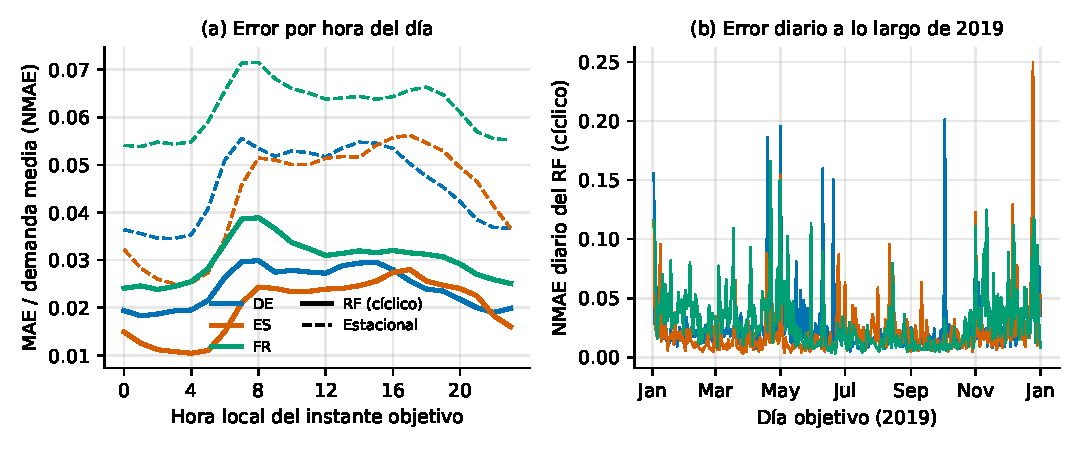
\includegraphics[width=0.86\textwidth]{img/fig_diagnostico.pdf}
\end{figure}

\begin{table}[!htbp]
    \centering
        \caption{Error del Random Forest cíclico en 2019 por subgrupo: tamaño ($n$), MAE (MW) y reducción del MAE frente a la referencia semanal.\label{tab:diag}}
        \footnotesize
        \resizebox{\textwidth}{!}{\begin{tabular}{lrrrrrrrrr}
\toprule
 & \multicolumn{3}{c}{DE} & \multicolumn{3}{c}{ES} & \multicolumn{3}{c}{FR} \\
\cmidrule(lr){2-4}\cmidrule(lr){5-7}\cmidrule(lr){8-10}
Subgrupo & $n$ & MAE RF & Mejora & $n$ & MAE RF & Mejora & $n$ & MAE RF & Mejora \\
\midrule
Laborable & 6\,240 & 1\,489 & 49\% & 6\,240 & 656 & 54\% & 6\,111 & 1\,679 & 54\% \\
Fin de semana & 2\,496 & 1\,022 & 39\% & 2\,496 & 401 & 53\% & 2\,448 & 1\,493 & 44\% \\
\midrule
Invierno & 2\,136 & 1\,549 & 54\% & 2\,136 & 763 & 52\% & 2\,136 & 2\,293 & 55\% \\
Primavera & 2\,207 & 1\,659 & 41\% & 2\,207 & 464 & 56\% & 2\,207 & 2\,034 & 38\% \\
Verano & 2\,208 & 1\,086 & 50\% & 2\,208 & 617 & 52\% & 2\,031 & 879 & 55\% \\
Otoño & 2\,185 & 1\,132 & 41\% & 2\,185 & 492 & 56\% & 2\,185 & 1\,256 & 57\% \\
\midrule
Alta ($>$ p90) & 882 & 1\,415 & 49\% & 796 & 741 & 59\% & 782 & 2\,350 & 60\% \\
Resto & 7\,854 & 1\,349 & 47\% & 7\,940 & 567 & 53\% & 7\,777 & 1\,553 & 50\% \\
\bottomrule
\end{tabular}}
    \\ Alta demanda: respuesta sobre el percentil 90 de entrenamiento de cada país.
\end{table}

El modelo supera a la referencia en las 24 horas de los tres países (figura \ref{img:diagnostico}a), con menor error de madrugada y máximos entre las 8 y las 17 h. La ventaja se mantiene en laborables y fines de semana y en las cuatro estaciones, con reducciones del MAE de 38\,\% a 57\,\%; las menores son primavera en Francia (38\,\%), fin de semana en Alemania (39\,\%) y primavera en Alemania (41\,\%). En horas de alta demanda la reducción es de 49\,\% en DE, 59\,\% en ES y 60\,\% en FR, pero el modelo \textbf{subestima} (sesgo medio de $-745$, $-456$ y $-920$ MW): quien dimensione capacidad con él quedaría corto justo cuando la demanda es mayor.

\textbf{Extremos y situación no confiable.} Los peores días son feriados nacionales (anexo, tabla \ref{tab:peores}): el MAE diario llega a 3\,700--11\,200 MW entre los tres peores de cada país, y el modelo los sobreestima (figura \ref{img:diagnostico}b). El 2 de enero en los tres países y el 26 de diciembre en Francia, también entre los peores, se subestiman, de acuerdo con que el modelo usa la demanda deprimida del día anterior. En feriados la referencia semanal tampoco es confiable y a veces es mejor (1 de mayo y 11 de noviembre en Francia; 6 de diciembre en España). \emph{Por tanto, no se recomienda confiar en la predicción para feriados ni para el día siguiente a uno prolongado.} Si faltan horas dentro de las últimas 168, no hay media móvil semanal y no puede emitirse la predicción (1,4\,\% de las filas del periodo de desarrollo, 2015--2018).

\section{Discusión}

\textbf{Respuesta a la pregunta.} Un modelo con rezagos, medias móviles y calendario reduce a la mitad el error relativo de la predicción a 24 horas frente a la referencia estacional semanal: en 2019, el Random Forest cíclico obtiene un NMAE macro de 0,0249 frente a 0,0505 (50,7\,\% menos; IC 95\,\% de 45,4\,\% a 54,9\,\%), con mejoras de 47\,\% a 54\,\% en cada país, y en el periodo de desarrollo (2015--2018) la mejora fue similar (49,6\,\%) y consistente en las tres ventanas. Buena parte de la señal ya está en el patrón semanal (\texttt{lag\_168h} concentra 65\,\% de la importancia); los modelos agregan sobre todo su corrección con el nivel reciente.

\textbf{¿Justifica la ganancia la complejidad?} En 2019, Ridge mejora a la referencia 18,8\,\%, el árbol podado 34,1\,\% y el Random Forest 50,7\,\%. La ventaja del bosque sobre el árbol (25,1\,\%; IC de 22,6\,\% a 27,7\,\%) y sobre Ridge (39,2\,\%; IC de 36,4\,\% a 42,1\,\%) es clara en los intervalos por bloques, aunque condicionales al ajuste y a un solo año. Su costo es menor interpretabilidad, 200 árboles con millones de nodos, ajustes de segundos (8,5 s el modelo final) y mayor dependencia de la historia (con solo el último año de entrenamiento el error sube 8,3\,\%). Con reajuste periódico ese costo es razonable; si se requiriera un modelo simple y auditable, el árbol podado conserva dos tercios de la mejora (34,1\,\% frente a 50,7\,\%). El calendario cíclico agrega una ganancia pequeña pero distinguible del ruido (4,8\,\%; IC de 3,1\,\% a 6,7\,\%).

\textbf{Límites de generalización.}
\begin{itemize}
    \item Los resultados valen para Alemania, España y Francia en 2015--2019, no para otros países ni para cambios de régimen; los árboles no extrapolan niveles fuera del rango de entrenamiento. La evaluación final usa un solo año, y los intervalos no incluyen la variabilidad entre años ni la de reajustar.
    \item Se predice de forma sucesiva a horizonte fijo, no emitiendo todo el día siguiente a una hora de mercado. No hay temperatura ni feriados: los peores días de 2019 son feriados (hasta 11\,200 MW de MAE diario), y en alta demanda el modelo subestima (sesgo de $-456$ a $-920$ MW).
    \item La importancia de variables es asociación predictiva, no causalidad. Las cifras del periodo de desarrollo (2015--2018) incluyen el efecto de elegir hiperparámetros con las mismas ventanas; la estimación imparcial es la de 2019. La versión cíclica usa hiperparámetros buscados con indicadores, y la grilla de poda y la de \texttt{max\_features} del bosque tienen sus mejores valores en el borde (Métodos).
    \item Las ausentes se tratan con casos completos y no son homogéneas entre países (Francia pierde 2,5\,\% de las filas); evaluar en fechas comunes cambia poco el NMAE, pero no se descarta que sean sistemáticas.
\end{itemize}

\textbf{Condiciones para usar el modelo.} Requiere las últimas 168 horas de demanda sin faltantes y el calendario local del instante objetivo. Debe reentrenarse con datos recientes y toda la historia, y vigilarse frente a la referencia semanal. No se recomienda confiar en él para feriados ni para el día siguiente a uno prolongado (por ejemplo, el 2 de enero), donde el error diario puede ser varias veces el habitual, ni para dimensionar capacidad en demanda extrema, que tiende a subestimar. Un calendario de feriados sería la primera mejora a evaluar.

\section{Reproducibilidad y contribuciones}

\subsection{Comando, entradas y ejecución} \label{sec:repro}

El código está en el repositorio público del grupo (https://github.com/jorge-mardones-data/electricity-demand-forecasting.git), versión \pend{commit de la entrega final}. La única entrada es el paquete del caso (\texttt{data/raw/demanda\_horaria.csv}). Con XeLaTeX instalado (no se instala con \texttt{pip}), desde la raíz:
\begin{verbatim}
python -m pip install -r requirements.txt
python analisis.py
\end{verbatim}
\texttt{analisis.py} ejecuta auditoría, base analítica, validación (con los hiperparámetros fijados), sensibilidades, evaluación en 2019, bootstrap, diagnóstico, tablas, figuras y la compilación de este informe; \texttt{--busqueda-completa} repite la búsqueda de hiperparámetros (varias horas). Registra entorno y tiempos en \texttt{results/run\_info.json} y la diferencia con los resultados previos en \texttt{results/concordancia.csv}.

\textbf{Ejecuciones.} Los resultados provienen de una ejecución completa el 9 de noviembre de 2026 en un solo computador (Computadora A): Windows 11, Intel Core i5-14600K (20 núcleos lógicos), 31.7 GB de RAM, Python 3.11.9, NumPy 2.4.6, pandas 2.3.3, scikit-learn 1.7.2 (Pedregosa et al., 2011) y matplotlib 3.10.7, con semillas fijas (\texttt{random\_state} $=42$). La ejecución tardó 12.2 minutos, y la búsqueda de hiperparámetros del Random Forest, fuera de ella, 178 minutos. El 10 de noviembre se repitió en la computadora de otro integrante (Computadora B: AMD Ryzen 9600X, 12 núcleos lógicos, Ubuntu 24.04 en WSL2): en CPU, los pasos 3 a 6 tardaron 10.6 minutos frente a 11.9 en A. En una GPU NVIDIA RTX 5060 de 8 GB no se aceleraron; fueron algo más lentos (anexo, tabla \ref{tab:tiempos_equipos}).

\textbf{Concordancia y copia limpia.} Frente a los resultados previos del repositorio (generados con los notebooks del grupo), las diferencias son menores a 1,4\,\% de la escala de cada archivo: solo cambia visiblemente el Random Forest cíclico de 2019 (NMAE macro de 0,02493 a 0,02490), plausiblemente por cálculos de punto flotante (seno y coseno) distintos entre equipos o versiones de librerías, lo que no se verificó. El 9 de noviembre de 2026 se copió la carpeta (sin \texttt{.git} ni registros previos) a otra ubicación y se ejecutó \texttt{python analisis.py} en el mismo computador: terminó sin errores en 13,8 minutos con la misma concordancia. En B terminó sin errores y con diferencias menores a 1,4\,\%.

\subsection{Contribuciones del equipo}

\textbf{Jorge Mardones:} creación y estructuración del repositorio y todo el contenido de su primera versión (preparación y auditoría de los datos, base analítica, protocolo experimental, diseño de la validación y desarrollo de los modelos, notebooks 02 y 03). \textbf{Benjamín Ruiz:} secciones 3.3, 4.1 y 4.2 del enunciado (sensibilidades, evaluación en la reserva y métricas; notebooks 04 y 05 y \texttt{src/modeling.py}) y la ejecución de la comparación de modelos. \textbf{Matías Pineda:} redacción del informe e integración de todos los resultados, análisis complementarios (notebook 06), tablas y figuras (\texttt{src/make\_report\_assets.py}), \texttt{analisis.py}, \texttt{README.md} y \texttt{requirements.txt}. \textbf{Diego Paredes:} presentación del trabajo (\texttt{reports/presentacion/main.tex}, \texttt{style.tex} y \texttt{src/make\_presentation\_assets.py}, con sus figuras y tablas), revisión y corrección de detalles estructurales del informe, y verificar resultados.

\subsection{Declaración de uso de inteligencia artificial}

\textbf{Herramienta y fechas:} Claude Code (Anthropic), 8 y 9 de noviembre de 2026. \textbf{Propósito y partes afectadas:} borrador y recorte de este informe, integración de los resultados de 2019, bootstrap, diagnóstico y sensibilidades, \texttt{src/make\_report\_assets.py}, \texttt{src/run\_validation.py}, \texttt{analisis.py}, \texttt{README.md}, \texttt{requirements.txt}, el notebook 06, una celda de exportación en el notebook 03 y dos notas corregidas del notebook 05. \textbf{Comprobaciones:} tablas y figuras se generan desde \texttt{results/}; el bootstrap recalculado reproduce el del notebook 05; las cifras del texto se contrastaron con la ejecución única; \texttt{analisis.py} se ejecutó completo dos veces; los nombres de los feriados provienen del calendario oficial. Los borradores contenían errores de interpretación que la revisión detectó (sección 3.3).

\textbf{Herramienta y fechas:} ChatGPT (OpenAI), 4-8 de noviembre de 2026. \textbf{Propósito y partes afectadas:} herramienta de apoyo para estructura del repositorio inicial, exploración y auditoria de datos, construcción de la base analítica, desarrollo computacional en evaluacion y comparación de los cinco modelos iniciales. Se usó códigos principalmente en \texttt{docs/protocolo\_experimental.md}, en \texttt{src/audit\_data.py}, \texttt{src/build\_dataset.py} y en \texttt{notebooks/02\_experimental\_design.ipynb} y \texttt{notebooks/03\_model\_development.ipynb}. Los códigos y cualquier tipo de sugerencia fué revisada y adaptada por Jorge Mardones, responsable de las decisiones metodológicas iniciales del proyecto.

\textbf{Herramienta y fechas:} Claude Code (Anthropic), 8-10 de noviembre de 2026. \textbf{Propósito y partes afectadas:} Diseño, cohesión y estructura de presentación (\texttt{reports/presentacion/main.tex} y \texttt{style.tex}) a partir de los resultados obtenidos, y creación de \texttt{src/make\_presentation\_assets.py} para generar figuras y tablas con formatos aptos para exposición en sala. Revisión y corrección de la estructura de flotantes que desplazaban secciones del anexo técnico, y generación de la tabla de sensibilidad por país agregada a \texttt{make\_report\_assets.py}, para luego incluirla en el anexo (\texttt{content/anexo.tex}, \texttt{style.cls})

\textbf{Herramienta y fechas:} Claude (Anthropic, modo Cowork), 8--10 de noviembre de 2026: primera versión de los notebooks 04 y 05 y de \texttt{src/modeling.py} (verificado: reproduce el NMAE del notebook 03) y medición de tiempos CPU/GPU.



%%%%%%%%%%%%%%%%% BIBLIOGRAFIA %%%%%%%%%%%%%%%%%
\newpage
\indent
\section{Referencias bibliográficas}
\leftskip 0.3in
\parindent -0.3in

%%%%%%%%%%%%%%% ESCRIBIR DEBAJO EN FORMATO APA %%%%%%%%%%%%%%%
% las lineas de arriba permiten que tenga una sangría francesa.

Bergmeir, C., \& Benítez, J. M. (2012). On the use of cross-validation for time series predictor evaluation. \textit{Information Sciences, 191}, 192--213.

Breiman, L. (2001). Random forests. \textit{Machine Learning, 45}(1), 5--32.

Breiman, L., Friedman, J. H., Olshen, R. A., \& Stone, C. J. (1984). \textit{Classification and regression trees}. Wadsworth.

ENTSO-E. (s.\,f.). \textit{ENTSO-E Transparency Platform} [Plataforma de datos]. https://transparency.entsoe.eu/

Hoerl, A. E., \& Kennard, R. W. (1970). Ridge regression: Biased estimation for nonorthogonal problems. \textit{Technometrics, 12}(1), 55--67.

Hyndman, R. J., \& Athanasopoulos, G. (2021). \textit{Forecasting: Principles and practice} (3.ª ed.). OTexts. https://otexts.com/fpp3/

James, G., Witten, D., Hastie, T., \& Tibshirani, R. (2021). \textit{An introduction to statistical learning: With applications in R} (2.ª ed.). Springer.

Künsch, H. R. (1989). The jackknife and the bootstrap for general stationary observations. \textit{The Annals of Statistics, 17}(3), 1217--1241.

Open Power System Data. (2020). \textit{Data package Time series} (Versión 2020-10-06) [Conjunto de datos]. https://doi.org/10.25832/time\_series/2020-10-06

Pedregosa, F., Varoquaux, G., Gramfort, A., Michel, V., Thirion, B., Grisel, O., Blondel, M., Prettenhofer, P., Weiss, R., Dubourg, V., Vanderplas, J., Passos, A., Cournapeau, D., Brucher, M., Perrot, M., \& Duchesnay, É. (2011). Scikit-learn: Machine learning in Python. \textit{Journal of Machine Learning Research, 12}, 2825--2830.

\par
\leftskip 0pt
\parindent 0pt


%%%%%%%%%%%%%%%%% ANEXO TECNICO (max. 6 paginas) %%%%%%%%%%%%%%%%%

\newpage
\section{Anexo técnico}

\subsection{Descripción de la respuesta}

\begin{table}[!htbp]
    \centering
    \caption{Descripción de la demanda a 24 horas (MW), periodo de desarrollo 2015--2018.}
    \small
    \label{tab:respuesta}
    \begin{tabular}{lrrrrrr}
\toprule
País & $n$ & Media & Desv. est. & Mínimo & Mediana & Máximo \\
\midrule
DE & 35\,040 & 55\,834 & 10\,032 & 31\,307 & 55\,471 & 77\,549 \\
ES & 35\,023 & 28\,702 & 4\,575 & 18\,041 & 28\,905 & 41\,015 \\
FR & 35\,016 & 54\,069 & 11\,732 & 30\,426 & 52\,383 & 94\,492 \\
\bottomrule
\end{tabular}
    \\ \textit{\scriptsize{Calculada solo con respuestas observadas del periodo de desarrollo (2015--2018).}}
\end{table}

\begin{figure}[!htbp]
    \centering
        \caption{Perfil medio de la demanda a 24 horas por hora local, día de la semana (L = lunes) y mes del instante objetivo, relativo a la media de cada país (adimensional). Periodo de desarrollo (2015--2018).\label{img:descriptiva}}
        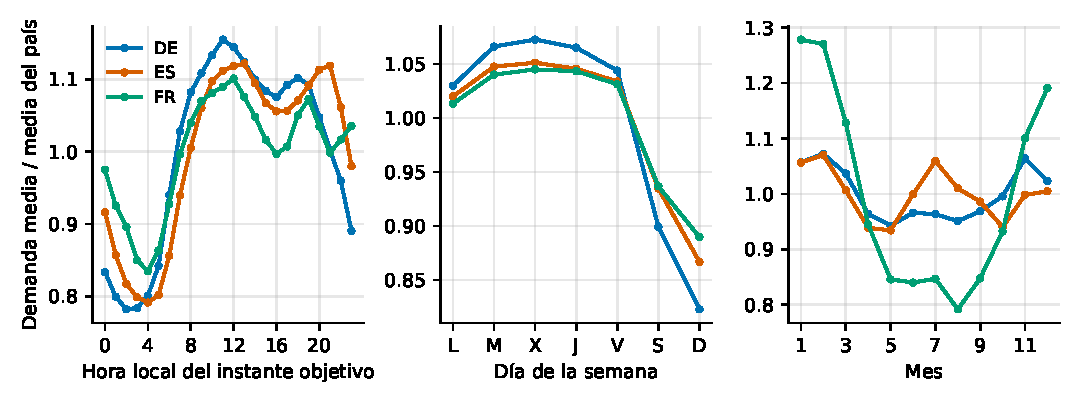
\includegraphics[width=0.95\textwidth]{img/fig_descriptiva.pdf}
\end{figure}

\subsection{Resultados completos de validación}

\begin{table}[!htbp]
    \centering
        \caption{MAE y RMSE (MW) y NMAE por procedimiento, ventana y país; NMAE macro en la última columna.\label{tab:detalle}}
        \resizebox{\textwidth}{!}{\begin{tabular}{llrrrrrrrrrr}
\toprule
 & & \multicolumn{3}{c}{DE} & \multicolumn{3}{c}{ES} & \multicolumn{3}{c}{FR} & Macro \\
\cmidrule(lr){3-5}\cmidrule(lr){6-8}\cmidrule(lr){9-11}
Procedimiento & Ventana & MAE & RMSE & NMAE & MAE & RMSE & NMAE & MAE & RMSE & NMAE & NMAE \\
\midrule
Persistencia & W1 & 4\,492 & 7\,018 & 0{,}0820 & 1\,790 & 2\,760 & 0{,}0630 & 3\,091 & 4\,592 & 0{,}0580 & 0{,}0677 \\
 & W2 & 4\,550 & 7\,007 & 0{,}0826 & 1\,842 & 2\,781 & 0{,}0647 & 3\,023 & 4\,443 & 0{,}0561 & 0{,}0678 \\
 & W3 & 4\,616 & 7\,026 & 0{,}0832 & 1\,824 & 2\,829 & 0{,}0638 & 3\,122 & 4\,575 & 0{,}0579 & 0{,}0683 \\
\midrule
Estacional semanal & W1 & 2\,208 & 4\,006 & 0{,}0403 & 1\,285 & 2\,014 & 0{,}0453 & 3\,458 & 4\,974 & 0{,}0648 & 0{,}0501 \\
 & W2 & 2\,441 & 4\,413 & 0{,}0443 & 1\,458 & 2\,140 & 0{,}0512 & 3\,606 & 5\,161 & 0{,}0669 & 0{,}0542 \\
 & W3 & 2\,557 & 4\,368 & 0{,}0461 & 1\,347 & 2\,111 & 0{,}0471 & 4\,185 & 6\,058 & 0{,}0776 & 0{,}0569 \\
\midrule
M1: Ridge & W1 & 2\,240 & 3\,318 & 0{,}0409 & 1\,157 & 1\,627 & 0{,}0407 & 2\,317 & 3\,204 & 0{,}0434 & 0{,}0417 \\
 & W2 & 2\,325 & 3\,477 & 0{,}0422 & 1\,256 & 1\,752 & 0{,}0441 & 2\,259 & 3\,100 & 0{,}0419 & 0{,}0428 \\
 & W3 & 2\,374 & 3\,458 & 0{,}0428 & 1\,233 & 1\,702 & 0{,}0431 & 2\,489 & 3\,477 & 0{,}0461 & 0{,}0440 \\
\midrule
M2: Árbol podado & W1 & 1\,795 & 3\,158 & 0{,}0328 & 998 & 1\,643 & 0{,}0351 & 2\,326 & 3\,473 & 0{,}0436 & 0{,}0372 \\
 & W2 & 1\,953 & 3\,484 & 0{,}0354 & 960 & 1\,563 & 0{,}0338 & 2\,138 & 3\,225 & 0{,}0397 & 0{,}0363 \\
 & W3 & 1\,819 & 3\,181 & 0{,}0328 & 814 & 1\,404 & 0{,}0285 & 2\,318 & 3\,516 & 0{,}0430 & 0{,}0347 \\
\midrule
M3: Random Forest (dummies) & W1 & 1\,430 & 2\,464 & 0{,}0261 & 755 & 1\,201 & 0{,}0266 & 1\,798 & 2\,700 & 0{,}0337 & 0{,}0288 \\
 & W2 & 1\,537 & 2\,598 & 0{,}0279 & 750 & 1\,214 & 0{,}0264 & 1\,700 & 2\,487 & 0{,}0316 & 0{,}0286 \\
 & W3 & 1\,461 & 2\,395 & 0{,}0263 & 627 & 1\,090 & 0{,}0219 & 1\,805 & 2\,704 & 0{,}0335 & 0{,}0272 \\
\bottomrule
\end{tabular}}
\end{table}

\subsection{Búsqueda de hiperparámetros}

\begin{table}[!htbp]
    \centering
        \caption{Ridge: NMAE macro medio y desviación estándar entre ventanas por valor de $\alpha$ (ordenado por NMAE).\label{tab:ridge}}
        \small
        \begin{tabular}{rrr@{\hspace{1cm}}rrr}
\toprule
$\alpha$ & Media & Desv. est. & $\alpha$ & Media & Desv. est. \\
\midrule
316{,}23 & 0{,}04282 & 0{,}00117 & $3{,}2\times10^{-2}$ & 0{,}04298 & 0{,}00114 \\
100{,}00 & 0{,}04283 & 0{,}00124 & $1{,}0\times10^{-2}$ & 0{,}04298 & 0{,}00114 \\
31{,}62 & 0{,}04291 & 0{,}00120 & $3{,}2\times10^{-3}$ & 0{,}04298 & 0{,}00114 \\
10{,}00 & 0{,}04296 & 0{,}00116 & $1{,}0\times10^{-3}$ & 0{,}04298 & 0{,}00114 \\
3{,}16 & 0{,}04297 & 0{,}00115 & 1\,000 & 0{,}04341 & 0{,}00069 \\
1{,}00 & 0{,}04298 & 0{,}00115 & 3\,162 & 0{,}04653 & 0{,}00195 \\
0{,}32 & 0{,}04298 & 0{,}00115 & 10\,000 & 0{,}05733 & 0{,}00763 \\
0{,}10 & 0{,}04298 & 0{,}00114 &  &  &  \\
\bottomrule
\end{tabular}
    \\ Entre $\alpha=0{,}001$ y $316$ el NMAE es prácticamente constante: el resultado es insensible al valor exacto.
\end{table}

\textbf{Random Forest.} Se evaluaron 18 configuraciones (200 árboles; profundidad máxima ninguna, 15 o 25; mínimo de observaciones por hoja 2, 5 o 10; fracción de predictores 0,7 o 1,0). La configuración seleccionada obtuvo 0,02821 (desviación estándar 0,00085; mínimo 0,02724 en W3 y máximo 0,02880 en W1). La siguiente mejor (profundidad máxima 25) difiere en solo 0,00001, por lo que ambas son prácticamente equivalentes. La tabla \ref{tab:rf_busqueda} entrega las 18 configuraciones.

\begin{table}[!htbp]
    \centering
        \caption{Random Forest: NMAE macro por configuración (promedio, desviación estándar, mínimo y máximo entre ventanas), ordenado por promedio. Todas con 200 árboles.\label{tab:rf_busqueda}}
        \small
        \begin{tabular}{rrrrrrr}
\toprule
\texttt{max\_depth} & \texttt{min\_samples\_leaf} & \texttt{max\_features} & Media & Desv. est. & Mínimo & Máximo \\
\midrule
ninguna & 2 & 0{,}7 & 0{,}02821 & 0{,}00085 & 0{,}02724 & 0{,}02880 \\
25 & 2 & 0{,}7 & 0{,}02822 & 0{,}00084 & 0{,}02726 & 0{,}02878 \\
15 & 2 & 0{,}7 & 0{,}02847 & 0{,}00072 & 0{,}02765 & 0{,}02890 \\
25 & 5 & 0{,}7 & 0{,}02853 & 0{,}00084 & 0{,}02756 & 0{,}02910 \\
ninguna & 5 & 0{,}7 & 0{,}02856 & 0{,}00084 & 0{,}02760 & 0{,}02912 \\
15 & 5 & 0{,}7 & 0{,}02869 & 0{,}00079 & 0{,}02778 & 0{,}02916 \\
ninguna & 2 & 1{,}0 & 0{,}02894 & 0{,}00100 & 0{,}02779 & 0{,}02962 \\
25 & 2 & 1{,}0 & 0{,}02894 & 0{,}00101 & 0{,}02779 & 0{,}02964 \\
15 & 2 & 1{,}0 & 0{,}02918 & 0{,}00088 & 0{,}02816 & 0{,}02969 \\
ninguna & 5 & 1{,}0 & 0{,}02919 & 0{,}00096 & 0{,}02809 & 0{,}02983 \\
25 & 5 & 1{,}0 & 0{,}02920 & 0{,}00096 & 0{,}02809 & 0{,}02984 \\
25 & 10 & 0{,}7 & 0{,}02920 & 0{,}00089 & 0{,}02818 & 0{,}02983 \\
ninguna & 10 & 0{,}7 & 0{,}02921 & 0{,}00089 & 0{,}02819 & 0{,}02983 \\
15 & 10 & 0{,}7 & 0{,}02927 & 0{,}00085 & 0{,}02829 & 0{,}02985 \\
15 & 5 & 1{,}0 & 0{,}02933 & 0{,}00088 & 0{,}02831 & 0{,}02986 \\
ninguna & 10 & 1{,}0 & 0{,}02973 & 0{,}00102 & 0{,}02856 & 0{,}03042 \\
25 & 10 & 1{,}0 & 0{,}02973 & 0{,}00102 & 0{,}02856 & 0{,}03042 \\
15 & 10 & 1{,}0 & 0{,}02979 & 0{,}00098 & 0{,}02866 & 0{,}03043 \\
\bottomrule
\end{tabular}
\end{table}

\subsection{Complejidad, costo e importancia del modelo final}

\begin{table}[!htbp]
    \centering
        \caption{Complejidad de los modelos finales ajustados con el periodo de desarrollo completo (2015--2018).\label{tab:complejidad}}
        \small
        \begin{tabular}{lrrrrr}
\toprule
Modelo final & Árboles & Profundidad media & Profundidad máxima & Nodos & Hojas \\
\midrule
Random Forest (cíclico) & 200 & 35{,}2 & 44 & 11\,412\,818 & 5\,706\,509 \\
Árbol podado & 1 & 26{,}0 & 26 & 8\,521 & 4\,261 \\
\bottomrule
\end{tabular}
\end{table}

\begin{table}[!htbp]
    \centering
        \caption{Tiempo de ajuste final de cada procedimiento con el periodo de desarrollo completo (2015--2018).\label{tab:tiempos}}
        \small
        \begin{tabular}{lr}
\toprule
Procedimiento & Ajuste final (s) \\
\midrule
M1: Ridge & 0{,}1 \\
M2: Árbol podado & 70{,}3 \\
M3: Random Forest (dummies) & 142{,}1 \\
M3$^\ast$: Random Forest (cíclico) & 8{,}5 \\
\bottomrule
\end{tabular}
\end{table}

\begin{table}[!htbp]
    \centering
        \caption{Importancia basada en impureza del Random Forest cíclico final (ajustado con 2015--2018), agrupada por predictor original (seno y coseno de una variable se suman).\label{tab:importancia}}
        \small
        \begin{tabular}{lr@{\hspace{1.2cm}}lr}
\toprule
Predictor & Importancia & Predictor & Importancia \\
\midrule
\texttt{lag\_168h} & 0{,}6468 & \texttt{rolling\_mean\_168h} & 0{,}0089 \\
\texttt{demand\_mw} & 0{,}2474 & \texttt{rolling\_mean\_24h} & 0{,}0083 \\
\texttt{lag\_48h} & 0{,}0499 & \texttt{target\_hour} & 0{,}0035 \\
\texttt{target\_day} & 0{,}0161 & \texttt{target\_month} & 0{,}0029 \\
\texttt{lag\_72h} & 0{,}0150 & \texttt{country} & 0{,}0012 \\
\bottomrule
\end{tabular}
\end{table}

\subsection{Incertidumbre y diagnóstico}

\begin{figure}[!htbp]
    \centering
        \caption{Distribución bootstrap de la diferencia de NMAE macro entre el Random Forest cíclico y la referencia estacional semanal (2\,000 réplicas por bloques semanales). Las líneas discontinuas marcan el intervalo de 95\,\%.\label{img:bootstrap}}
        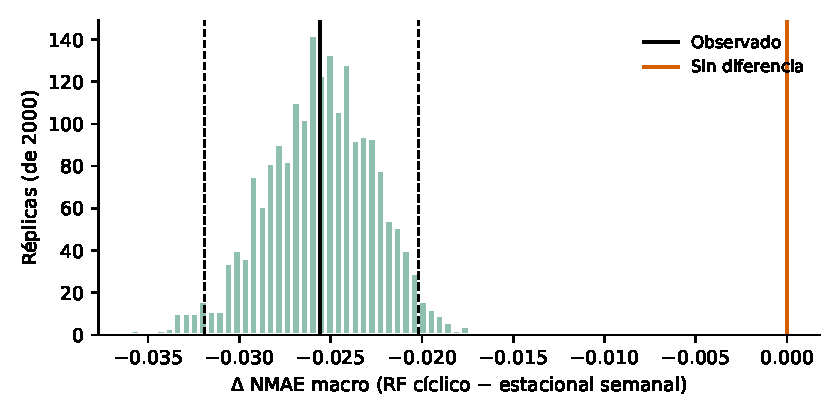
\includegraphics[width=0.62\textwidth]{img/fig_bootstrap.pdf}
\end{figure}

\begin{table}[!htbp]
    \centering
        \caption{Los tres días objetivo con mayor MAE diario del Random Forest cíclico en 2019, por país.\label{tab:peores}}
        \footnotesize
        \begin{tabular}{llp{4.2cm}rrr}
\toprule
País & Fecha objetivo & Feriado nacional & MAE RF (MW) & MAE estac. (MW) & Sesgo RF (MW) \\
\midrule
DE & 03-10-2019 & Día de la Unidad Alemana & 11\,240 & 12\,150 & 11\,240 \\
 & 01-05-2019 & Día del Trabajo & 10\,916 & 12\,761 & 10\,916 \\
 & 19-04-2019 & Viernes Santo & 10\,377 & 15\,033 & 10\,377 \\
\midrule
ES & 25-12-2019 & Navidad & 7\,168 & 10\,347 & 7\,168 \\
 & 01-05-2019 & Día del Trabajo & 4\,430 & 5\,954 & 4\,430 \\
 & 06-12-2019 & Día de la Constitución & 3\,712 & 2\,951 & 3\,633 \\
\midrule
FR & 22-04-2019 & Lunes de Pascua & 8\,962 & 15\,827 & 8\,962 \\
 & 01-05-2019 & Día del Trabajo & 8\,095 & 6\,685 & 8\,095 \\
 & 11-11-2019 & Armisticio & 6\,730 & 3\,645 & 6\,704 \\
\bottomrule
\end{tabular}
    \\ Sesgo = predicción menos observado (positivo: sobreestimación). Los nombres de los feriados provienen del calendario oficial, no de los datos.
\end{table}

\subsection{Resultados completos de la evaluación en 2019}

\begin{table}[!htbp]
    \centering
        \caption{MAE y RMSE (MW) y NMAE por procedimiento y país en la reserva 2019; NMAE macro en la última columna.\label{tab:test_detalle}}
        \resizebox{\textwidth}{!}{\begin{tabular}{lrrrrrrrrrr}
\toprule
 & \multicolumn{3}{c}{DE} & \multicolumn{3}{c}{ES} & \multicolumn{3}{c}{FR} & Macro \\
\cmidrule(lr){2-4}\cmidrule(lr){5-7}\cmidrule(lr){8-10}
Procedimiento & MAE & RMSE & NMAE & MAE & RMSE & NMAE & MAE & RMSE & NMAE & NMAE \\
\midrule
Persistencia & 4\,563 & 6\,951 & 0{,}0817 & 1\,777 & 2\,707 & 0{,}0619 & 3\,098 & 4\,529 & 0{,}0574 & 0{,}0670 \\
\midrule
Estacional semanal & 2\,559 & 4\,469 & 0{,}0458 & 1\,255 & 2\,002 & 0{,}0437 & 3\,337 & 4\,635 & 0{,}0618 & 0{,}0505 \\
\midrule
M1: Ridge & 2\,336 & 3\,462 & 0{,}0418 & 1\,220 & 1\,672 & 0{,}0425 & 2\,084 & 2\,836 & 0{,}0386 & 0{,}0410 \\
\midrule
M2: Árbol podado & 1\,780 & 3\,145 & 0{,}0319 & 785 & 1\,293 & 0{,}0273 & 2\,189 & 3\,317 & 0{,}0406 & 0{,}0333 \\
\midrule
M3: Random Forest (dummies) & 1\,438 & 2\,386 & 0{,}0257 & 611 & 1\,047 & 0{,}0213 & 1\,697 & 2\,507 & 0{,}0314 & 0{,}0262 \\
\midrule
M3$^\ast$: Random Forest (cíclico) & 1\,355 & 2\,227 & 0{,}0243 & 583 & 1\,015 & 0{,}0203 & 1\,626 & 2\,403 & 0{,}0301 & 0{,}0249 \\
\bottomrule
\end{tabular}}
\end{table}

\subsection{Correlación entre predictores}

\begin{table}[!htbp]
    \centering
        \caption{Correlación de Pearson entre los predictores numéricos y la respuesta en el entrenamiento final (2015--2018), calculada dentro de cada país y promediada entre los tres.\label{tab:correlacion}}
        \footnotesize
        \resizebox{\textwidth}{!}{\begin{tabular}{lrrrrrr}
\toprule
 & \texttt{demand\_mw} & \texttt{lag\_48h} & \texttt{lag\_72h} & \texttt{lag\_168h} & \texttt{rolling\_mean\_24h} & \texttt{rolling\_mean\_168h} \\
\midrule
\texttt{lag\_48h} & 0{,}83 &  &  &  &  &  \\
\texttt{lag\_72h} & 0{,}67 & 0{,}83 &  &  &  &  \\
\texttt{lag\_168h} & 0{,}78 & 0{,}64 & 0{,}61 &  &  &  \\
\texttt{rolling\_mean\_24h} & 0{,}67 & 0{,}66 & 0{,}41 & 0{,}37 &  &  \\
\texttt{rolling\_mean\_168h} & 0{,}50 & 0{,}52 & 0{,}53 & 0{,}52 & 0{,}69 &  \\
\texttt{target\_demand\_mw} & 0{,}83 & 0{,}67 & 0{,}62 & 0{,}91 & 0{,}43 & 0{,}48 \\
\bottomrule
\end{tabular}}
    \\ La última fila es la correlación con la respuesta \texttt{target\_demand\_mw}.
\end{table}

\subsection{Datos ausentes}

\begin{table}[!htbp]
    \centering
        \caption{Bloques de horas consecutivas sin demanda observada, por país (2015--2019).\label{tab:ausentes_bloques}}
        \small
        \begin{tabular}{llrr}
\toprule
País & Fecha de inicio (UTC) & Hora & Horas consecutivas \\
\midrule
DE & sin ausentes & -- & 0 \\
\midrule
ES & 01-01-2015 & 00:00 & 1 \\
 & 02-01-2015 & 06:00 & 3 \\
 & 02-01-2015 & 11:00 & 8 \\
 & 01-05-2015 & 10:00 & 6 \\
\midrule
FR & 01-01-2015 & 00:00 & 1 \\
 & 05-02-2017 & 19:00 & 13 \\
 & 12-08-2018 & 07:00 & 5 \\
 & 04-10-2018 & 01:00 & 3 \\
 & 14-12-2018 & 04:00 & 3 \\
 & 25-07-2019 & 00:00 & 5 \\
\bottomrule
\end{tabular}
\end{table}

\begin{table}[!htbp]
    \centering
        \caption{NMAE de cada país con sus casos completos (propio) y restringido a las fechas en que los tres países tienen caso completo (común).\label{tab:ausentes_efecto}}
        \footnotesize
        \resizebox{\textwidth}{!}{\begin{tabular}{llrrrrrrrr}
\toprule
 & & \multicolumn{2}{c}{$n$} & \multicolumn{2}{c}{Estacional} & \multicolumn{2}{c}{Ridge} & \multicolumn{2}{c}{RF cíclico} \\
\cmidrule(lr){3-4}\cmidrule(lr){5-6}\cmidrule(lr){7-8}\cmidrule(lr){9-10}
Periodo & País & Propio & Común & Propio & Común & Propio & Común & Propio & Común \\
\midrule
W1 & DE & 8\,784 & 8\,784 & 0{,}0403 & 0{,}0403 & 0{,}0409 & 0{,}0409 & -- & -- \\
 & ES & 8\,784 & 8\,784 & 0{,}0453 & 0{,}0453 & 0{,}0407 & 0{,}0407 & -- & -- \\
 & FR & 8\,784 & 8\,784 & 0{,}0648 & 0{,}0648 & 0{,}0434 & 0{,}0434 & -- & -- \\
 & Macro & 26\,352 & 26\,352 & 0{,}0501 & 0{,}0501 & 0{,}0417 & 0{,}0417 & -- & -- \\
\midrule
W2 & DE & 8\,760 & 8\,567 & 0{,}0443 & 0{,}0447 & 0{,}0422 & 0{,}0424 & -- & -- \\
 & ES & 8\,760 & 8\,567 & 0{,}0512 & 0{,}0518 & 0{,}0441 & 0{,}0442 & -- & -- \\
 & FR & 8\,567 & 8\,567 & 0{,}0669 & 0{,}0669 & 0{,}0419 & 0{,}0419 & -- & -- \\
 & Macro & 26\,087 & 25\,701 & 0{,}0542 & 0{,}0545 & 0{,}0428 & 0{,}0429 & -- & -- \\
\midrule
W3 & DE & 8\,736 & 8\,213 & 0{,}0461 & 0{,}0463 & 0{,}0428 & 0{,}0434 & -- & -- \\
 & ES & 8\,736 & 8\,213 & 0{,}0471 & 0{,}0465 & 0{,}0431 & 0{,}0430 & -- & -- \\
 & FR & 8\,213 & 8\,213 & 0{,}0776 & 0{,}0776 & 0{,}0461 & 0{,}0461 & -- & -- \\
 & Macro & 25\,685 & 24\,639 & 0{,}0569 & 0{,}0568 & 0{,}0440 & 0{,}0442 & -- & -- \\
\midrule
2019 & DE & 8\,736 & 8\,559 & 0{,}0458 & 0{,}0463 & 0{,}0418 & 0{,}0420 & 0{,}0243 & 0{,}0244 \\
 & ES & 8\,736 & 8\,559 & 0{,}0437 & 0{,}0429 & 0{,}0425 & 0{,}0425 & 0{,}0203 & 0{,}0201 \\
 & FR & 8\,559 & 8\,559 & 0{,}0618 & 0{,}0618 & 0{,}0386 & 0{,}0386 & 0{,}0301 & 0{,}0301 \\
 & Macro & 26\,031 & 25\,677 & 0{,}0505 & 0{,}0503 & 0{,}0410 & 0{,}0410 & 0{,}0249 & 0{,}0249 \\
\bottomrule
\end{tabular}}
    \\ Estacional: referencia estacional semanal. $n$ corresponde a las filas de evaluación del país (en Macro, suma de los tres). Para Francia ambos valores coinciden porque sus fechas son un subconjunto de las de los otros países. El Random Forest cíclico solo se evalúa en 2019.
\end{table}

\pend{PENDIENTE: Agregar al anexo los resultados de las sensibilidades por país.}

\subsection{Costo computacional: CPU frente a GPU} \label{sec:gpu}

Se midió el tiempo de reloj de cada sección de los notebooks y de la validación (\texttt{src/timing.py}) en un computador con CPU AMD Ryzen 5 9600X (12 núcleos lógicos) y GPU NVIDIA RTX 5060 (8 GB), en Ubuntu 24.04 (WSL2), y se repitió con la GPU mediante RAPIDS cuML (\texttt{docs/tiempos\_cpu\_gpu.md}). Es una sola ejecución por configuración, sin repeticiones, por lo que las diferencias pequeñas no son concluyentes.

\textbf{Acelerador automático} (\texttt{cuml.accel}, \texttt{analisis.py --gpu}). Los pasos 3 a 6 tardaron 633 s en CPU y 719 s con GPU (0,88 veces la velocidad de la CPU). Ridge sí se ejecutó en la GPU, pero su primer ajuste pagó 13 s de inicialización; el árbol podado y el Random Forest con indicadores casi no cambiaron de tiempo (134 frente a 139 s en W1--W3), lo que sugiere que siguieron en CPU: cuML no tiene árbol con poda, y una explicación plausible, no verificada, para el bosque es que la codificación con indicadores produce una matriz dispersa.

\textbf{Modelos forzados a la GPU} (\texttt{src/benchmark\_gpu.py}, solo W1--W3). Se ajustaron directamente con cuML, con matriz densa en \texttt{float32} (tabla \ref{tab:gpu}). cuML exige una profundidad máxima finita, por lo que se comparó con scikit-learn con la misma profundidad.

\begin{table}[!htbp]
    \centering
        \caption{Ajuste y predicción en W1--W3 (suma de segundos) y NMAE macro medio, CPU (scikit-learn) frente a GPU (cuML), con matriz densa.\label{tab:gpu}}
        \footnotesize
        \begin{tabular}{@{}lrrrrr@{}}
            \toprule
            Modelo & CPU (s) & GPU (s) & Velocidad GPU/CPU & NMAE CPU & NMAE GPU \\
            \midrule
            Ridge & 0,04 & 0,10 & 0,43 & 0,04282 & 0,04282 \\
            RF indicadores, profundidad 16 & 15,5 & 26,4 & 0,59 & 0,02832 & 0,02844 \\
            RF indicadores, profundidad 32 & 18,6 & 59,7 & 0,31 & 0,02820 & 0,02830 \\
            RF cíclico, profundidad 16 & 13,5 & 15,7 & 0,86 & 0,02716 & 0,02724 \\
            RF cíclico, profundidad 32 & 15,6 & 33,5 & 0,47 & 0,02711 & 0,02722 \\
            \midrule
            RF indicadores, sin límite (oficial) & 18,2 & -- & -- & 0,02821 & -- \\
            \bottomrule
        \end{tabular}
    \\ Velocidad GPU/CPU $<1$: la GPU es más lenta. Excluye 10 s de inicialización de la GPU.
\end{table}

La GPU fue más lenta en todos los casos, más aún con árboles profundos y con más columnas (indicadores), y el NMAE cambió menos de 0,5\,\%. Su desventaja se reduce al crecer el entrenamiento (RF cíclico, profundidad 16: 0,52 en W1, 0,88 en W2 y 1,06 en W3), por lo que con muchas más filas podría convenir; con unas 100\,000, no. La ganancia relevante fue otra: el mismo Random Forest oficial con matriz densa tardó 18 s en W1--W3, frente a 134 s con la matriz dispersa del \textit{pipeline}, con igual NMAE (0,02821). Este cambio no se aplicó a los resultados del informe.



\end{document}